\documentclass[conference]{IEEEtran}
\IEEEoverridecommandlockouts
\usepackage{fancyhdr}
\usepackage[british]{babel}
\tolerance=1
\emergencystretch=\maxdimen
\hyphenpenalty=10000
\hbadness=10000

% Phil's macros
% Create code font alias
\usepackage{float}
\usepackage{tikz}
% Code
\usepackage{listings}
\usepackage{xcolor}
\newcommand{\code}[1]{\texttt{#1}}
\usepackage{minted}
\usepackage{algorithm}
\usepackage{standalone}
\usepackage{algorithmicx}
\usepackage[noend]{algpseudocode}
\usemintedstyle{trac}
\renewcommand\algorithmicdo{}
\renewcommand\algorithmicthen{}
\setlength{\parindent}{0em}

\usepackage{setspace}
\renewcommand{\baselinestretch}{1.35}


\pagestyle{fancy}
\fancyhead{}

\lstdefinestyle{customc}{
belowcaptionskip=1\baselineskip,
breaklines=true,
frame=L,
xleftmargin=\parindent,
language=C,
showstringspaces=false,
basicstyle=\footnotesize\ttfamily,
keywordstyle=\bfseries\color{green!40!black},
commentstyle=\itshape\color{purple!40!black},
identifierstyle=\color{blue},
stringstyle=\color{orange},
columns=fullflexible,
language=c,
frame=true,
numbers=left
}
\lstdefinestyle{snippet}{
belowcaptionskip=1\baselineskip,
breaklines=true,
frame=L,
xleftmargin=\parindent,
language=C,
showstringspaces=false,
basicstyle=\footnotesize\ttfamily,
keywordstyle=\bfseries\color{green!40!black},
commentstyle=\itshape\color{purple!40!black},
identifierstyle=\color{blue},
stringstyle=\color{orange},
columns=fullflexible,
language=c
}
\lstdefinestyle{hex}{
belowcaptionskip=1\baselineskip,
breaklines=true,
frame=LR,
% xleftmargin=\parindent,
language=C,
showstringspaces=false,
basicstyle=\footnotesize\ttfamily,
keywordstyle=\bfseries\color{green!40!black},
commentstyle=\itshape\color{purple!40!black},
% identifierstyle=\color{blue},
stringstyle=\color{orange},
columns=fullflexible,
keywords=[2]{fail},
keywords=[3]{pass},
keywordstyle={\color{blue!80!black}},
keywordstyle=[2]{\color{red!80!black}},
keywordstyle=[3]{\color{green!50!black}},
}

\lstdefinestyle{asm}{
belowcaptionskip=1\baselineskip,
keepspaces,
breaklines=true,
tabsize=8,
frame=L,
xleftmargin=\parindent,
language=[x86masm]Assembler,
showstringspaces=false,
basicstyle=\footnotesize\ttfamily,
keywordstyle=\bfseries\color{green!40!black},
commentstyle=\itshape\color{purple!40!black},
identifierstyle=\color{blue},
stringstyle=\color{orange},
columns=fullflexible,
}

% The preceding line is only needed to identify funding in the first footnote. If that is unneeded, please comment it out.
% \usepackage{cite}
\usepackage{amsmath,amssymb,amsfonts}
\usepackage{graphicx}
\usepackage{textcomp}
\def\BibTeX{{\rm B\kern-.05em{\sc i\kern-.025em b}\kern-.08em
T\kern-.1667em\lower.7ex\hbox{E}\kern-.125emX}}
\begin{document}

\title{Breaking Trivium with Stuck-at-0 Faults}

\author{\IEEEauthorblockN{Phillip Gajland}
\IEEEauthorblockA{\textit{KTH Royal Institute of Technology} \\
\textit{Theoretical Computer Science} \\
Stockholm, Sweden \\
gajland@kth.se}
}

\maketitle

\begin{abstract}
As the Internet of Things (IoT) continues to gain traction, so does the need for secure IoT devices. Although 23.3 billion IoT devices are estimated to be connected by 2023 \cite{iot}, vendors often neglect the security of such devices. Stream ciphers can offer an attractive solution for secure communications, when low power consumption is essential. 

The eSTREAM project was intended to \textit{"identify new stream ciphers suitable for widespread adoption"}.\cite{call} In 2008, Trivium, a synchronous stream cipher was selected as part of the portfolio for low area hardware ciphers. 

In this paper we study the design choices made by the authors of Trivium in order to demonstrate a fault attack on the software implementation of the cipher. Whilst Trivium maintains most desirable cryptographic properties, a simple design was chosen by the authors to provide flexibility. Our non-invasive attack works by modifying the compiled binary at targeted positions to introduce stuck-at-0 faults. Using this technique, we are able to reduce the non-linear feedback function to a linear one. Thus, it is possible to recover the 288-bit internal state of the cipher. In turn, extraction of the 80-bit key becomes tractable.
\end{abstract}

\begin{IEEEkeywords}
trivium, stream cipher, fault attack
\end{IEEEkeywords}

\section{Introduction}
As the Internet of Things (IoT) continues to gain traction, so does the need for secure IoT devices. Although 23.3 billion IoT devices are estimated to be connected by 2023 \cite{iot}, vendors often neglect the security of such devices. Thus, significantly increasing the attack surface for adversaries to mount attacks on larger systems. This was demonstrated in the 2016 Dyn cyberattack, when IoT devices where used as a botnet to perform a distributed denial of service attack \cite{dyn}. A primary concern is securing systems, and stream ciphers can offer an attractive solution for secure communications, when low power consumption is essential.

The eSTREAM project was intended to \textit{"identify new stream ciphers suitable for widespread adoption"}.\cite{call} In 2018, Trivium, a synchronous stream cipher was selected as part of the portfolio for low area hardware ciphers. In this paper we analyse the design choices made by the authors of Trivium, in order to reveal a new class of vulnerabilities in the cipher. We go on to demonstrate a fault attack on the software implementation of Trivium. The attack works by modifying compiled binaries at targeted positions to introduce stuck at 0 faults. Using this technique, we are able to reduce the non-linear feedback function to a linear one. Thus, it is possible to recover the 288-bit internal state of the cipher and in turn extraction of the 80-bit key becomes tractable.

The remainder of the paper is structured as follows. We start by giving a brief introduction to the eSTREAM project and Trivium's roots in Section \ref{sec:background}. Section \ref{sec:previous-work} gives an outline to some previous work. Section \ref{sec:spec} provides details to the Trivium design specification. Section \ref{sec:fault-inj} describes the fault injection attack. An analysis of the code and details as to how the attack is mounted is covered in Section \ref{sec:code}. A brief cryptanalysis follows in Section \ref{sec:cryptanalysis}.

\section{Background}\label{sec:background}

Already during World War II, the breaking of ciphers was of significant interest to the allied forces trying to intercept German communications. The work of Alan Turing amongst others at Bletchley Park, that led to breaking the Enigma Machine, has often been cited as an instrumental turning point which may have had a profound impact on the outcome of the war.
Although it was already known to the NSA at the time, another notable milestone in cryptography includes the discovery of Differential cryptanalysis on DES by Biham and Shamir \cite{des}. Over the years numerous creative attacks on ciphers have been proposed and techniques of fault injections date back to the 1970s \cite{history}. Whilst fault injections originated from hardware systems, today fault injections have become an attractive way to test both software and hardware systems under stress.

Stream ciphers are symmetric ciphers that make use of a pseudo random number generator, whose output is used as a keystream. For encryption, the keystream is XORed with the plaintext in order to obtain the cipher text. Decryption is done similarly; the ciphertext is XORed with the keystream in order to obtain the plaintext.

As a result of the failures of all six stream ciphers submitted to the NESSIE (New European Schemes for Signatures, Integrity and Encryption) project, the eSTREAM project was launched in 2004 in order to \textit{"identify new stream ciphers suitable for widespread adoption"} \cite{call}. Four years later, a portfolio of new stream ciphers was announced in April 2008. The portfolio was revised in September 2008, and currently consist of seven stream ciphers [See Table \ref{tab:portfolio}], divided into two profiles, hardware and software. The book entitled \textit{New Stream Cipher Designs - The eSTREAM Finalists} \cite{book} was published by Springer in 2008 and provides full specifications of all 16 ciphers that reached the final phase of the eSTREAM project.
\begin{table}[H]
\centering
\begin{tabular}{|l|l|}\hline
Profile 1 (Software) & Profile 2 (Hardware)\\\hline
HC-128 & Grain v1\\
Rabiit & MICKEY 2.0\\
Salsa20/12 & Trivium\\
SOSEMANUK & \\\hline
\end{tabular}
\caption{eSTREAM Portfolio}
\label{tab:portfolio}
\end{table}

\section{Previous Work}\label{sec:previous-work}

In this section we give an outline of some of the attacks aimed at Trivium. 
P. Hawkes and G. Rose showed guess-and-determine (GD) attacks on the SNOW stream cipher. A GD attack \textit{guesses} some internal values and then exploits the relationships to \textit{determine} other internal values; hence the name. However, this kind of attack is most suitable for word-oriented stream ciphers. The first attack has a data complexity of $2^{64}$ and a process complexity of $2^{256}$. That is, $2^{64}$ keystream bits are needed, whilst $2^{256}$ is the time complexity of processing the keystream in order to perform the attack. The second attack has a process complexity of $2^{224}$, and a data complexity of $2^{95}$.\cite{Hawkes2003}

In 2010 N. Rohani et al. showed a GD attack method on Trivium and Bivium \cite{Rohani2010} (Bivium is simply the truncated version of Trivium using two linear shift registers as opposed to three).
The attack works by guessing some of the internal state variables. Next, the remaining part of the internal state is determined based on the guesses and the outline of the cipher. Finally, assuming that the cipher is loaded with guessed and determined values, an output sequence is obtained from running the algorithm. This output sequence is compared with the actual output sequence. If the two sequences are identical, one can conclude that the guesses were correct. This process is continued with other guessed values until the output sequences match. Due to the large length of the internal state, the attack was not successful on Trivium. The complexity is of order $2^{90.67}$. However, for Bivium only $27.55$ bits need to be guessed in order to determine the remaining bits. A total of $2^{43.99}$ keystream bits are needed for the attack. The complexity of the attack on Bivium is $2^{27.55}$, which is an improvement to the previous GD attack demonstrated by McDonald, Charnes, Pieprzyk \cite{biv-old}, with a complexity of $2^{52.3}$.

M. Hojsík and B. Rudolf \cite{Hojsik2008} showed a Differential Fault Analysis of Trivium for which an attacker needs approximately 12 fault injections to obtain the secret key and IV. In their attack, the fault is injected into the inner state of the cipher. 
The attack essentially boils down to solving a system of equations in the inner state bits $IS_t = (s_1,\dots, s_{288})$
Their attack algorithm can be described as follows \cite{Hojsik2008}:
\begin{algorithmic}[1]
\State obtain the proper keystream generated from $IS_t$ 
\State insert the keystream equations into the system 
\While{solution not found}
\State reset the cipher to the state $IS_t$
\State insert a fault into $IS_t$ at random position
\State obtain the faulty keystream
\State determine the fault position
\State insert delta keystream equations into the system
\State try to solve the system
\EndWhile
\State clock Trivium backwards until initial state reached
\State read the secret key and IV
\end{algorithmic}

In 2012 Y. Hu et al. presented a fault analysis of Trivium \cite{Hu2012} with weaker assumptions than those required in \cite{Hojsik2008}. The authors present a novel checking method in which segments of the original keystream and fault injected keystream are compared, in order to determine the injection time and fault position. Their results, which are based on random simulations, show that for various distributions of injection times, Trivium can be broken with few repeated injections. By observing an average of $195 \times 17$ key-stream bits, the aforementioned attack can be done.

The attack presented in this paper is somewhat different to the aforementioned attacks, in that it uses a stuck-at-0 fault injected into the binary of Trivium. In 2019 Dubrova presented a similar attack on ACORN \cite{Dubrova}. The attack injects a single stuck-at-0 fault into the compiled binary of the cipher. With this fault, the key can be recovered from $2^{15.34}$ keystream bits using $2^{35.46}$ operations.

\section{Trivium Design Specification}\label{sec:spec}

Trivium is a synchronous stream cipher using an 80-bit key and a 80-bit initialisation vector (IV). The secret internal state consists of 288 bits and is made up of 3 registers of length 93, 84 and 111 bits [See Figure \ref{fig:circle}]. The cipher operation essentially consists of two phases; the key and IV setup as well as the keystream generation, which are described in Section \ref{sec:key-iv-o} and Section \ref{sec:key-gen-o} respectively.

\begin{figure}[H]
\centering
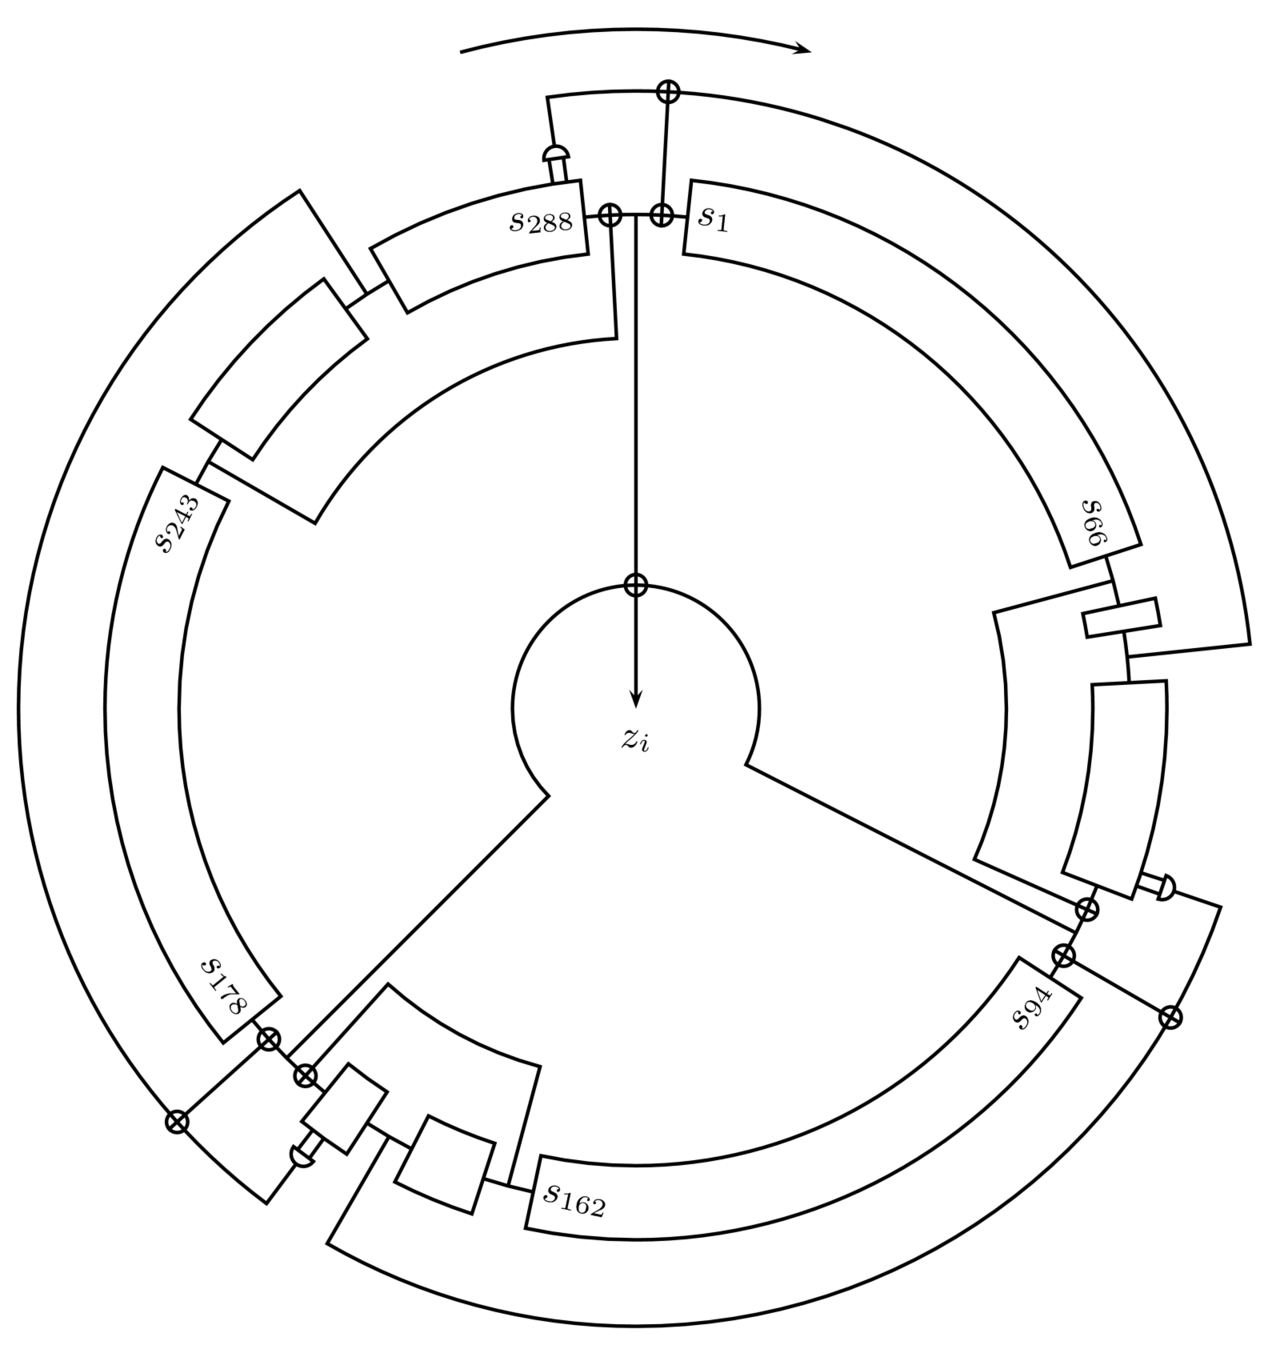
\includegraphics[width=0.45\textwidth]{figures/round.png}
\caption{Trivium \cite{circle}}
\label{fig:circle}
\end{figure}

\subsection{Keystream Generation}\label{sec:key-gen-o}
The keystream is generated as a linear combination of the three registers, $t_1\oplus t_2\oplus t_3=z_i$. At each clock cycle, three bits are updated using a non-linear feedback function, whilst one output bit $z_i$ is obtained [See Algorithm \ref{alg:orig} and Figure \ref{fig:original}]. The authors state in the cipher specification, that $2^{64}$ keystream bits can be obtained from a given Key/IV pair.

\begin{algorithm}[H]
\begin{algorithmic}[1]
\For{$i=1$ to $N$} \Comment{$N\leq 2^{64}$}
\State $t_1 \gets s_{66} + s_{93}$
\State $t_2 \gets s_{162} + s_{177}$
\State $t_3 \gets s_{243} + s_{288}$
\State
\State $z_i \gets t_1 + t_2 + t_3$
\State
\State $t_1 \gets t_1 + s_{91} \cdot s_{92} + s_{171}$
\State $t_2 \gets t_2 + s_{175} \cdot s_{176} + s_{264}$
\State $t_3 \gets t_3 + s_{286} \cdot s_{287} + s_{69}$
\State
\State $(s_1,s_2,\dots,s_{93}) \gets (t_3,s_1,\dots,s_{92})$
\State $(s_{94},s_{95},\dots,s_{177}) \gets (t_1,s_{94},\dots,s_{176})$
\State $(s_{178},s_{179},\dots,s_{288}) \gets (t_2,s_{178},\dots,s_{287})$
\EndFor
\end{algorithmic}
\caption{Original Keystream Generation}\label{alg:orig}
\end{algorithm}

\subsection{Key and IV Setup}\label{sec:key-iv-o}
The key is loaded into the first eighty bits of the first register, whilst the IV is loaded into the first eighty bits of the second register. All remaining bits are set to zero, with the exception of bits $s_{286},s_{287},s_{288}$ which are set to 1. The initialisation stage requires $4*288=1152$ steps and is identical to the keystream generation, except that there are no output bits [See Algorithm \ref{alg:orig-iv}].

\begin{algorithm}[H]
\begin{algorithmic}[1]
\State $(s_1,s_2,\dots,s_{93}) \gets (K_1,\dots,K_{80},0,\dots,0)$
\State $(s_{94},s_{95},\dots,s_{177}) \gets (IV_1,\dots,IV_{80},0,\dots,0)$
\State $(s_{178},s_{179},\dots,s_{288}) \gets (0,\dots,0,1,1,1)$
\State
\For{$i=1$ to $4\cdot288$}
\State $t_1 \gets s_{66} + s_{91} \cdot s_{92} + s_{93} + s_{171}$
\State $t_2 \gets s_{162} + s_{175} \cdot s_{176} + s_{177} + s_{264}$
\State $t_3 \gets s_{243} + s_{286} \cdot s_{287} + s_{288}+ s_{69}$
\State
\State $(s_1,s_2,\dots,s_{93}) \gets (t_3,s_1,\dots,s_{92})$
\State $(s_{94},s_{95},\dots,s_{177}) \gets (t_1,s_{94},\dots,s_{176})$
\State $(s_{178},s_{179},\dots,s_{288}) \gets (t_2,s_{178},\dots,s_{287})$
\EndFor
\end{algorithmic}
\caption{Original Key and IV Setup}\label{alg:orig-iv}
\end{algorithm}

\begin{figure}[H]
\centering
\includestandalone[width=0.45\textwidth]{figures/original}
\caption{Original Trivium}
\label{fig:original}
\end{figure}

\section{Fault Injection}\label{sec:fault-inj}

\subsection{Attack Scenario and Assumptions}\label{sec:fault}

We assume that the attacker has physical access to the device running Trivium. Given today's global supply chain, packages can easily be intercepted and tampered with during shipment. The attacker wishes to perform a non-invasive attack that leaves little traces of whether or not the micro-controller has been tampered with. Whilst the attack works similarly in hardware, for it to remain undetected we focus on the software implementation. There may be some proprietary protection mechanism, preventing arbitrary code from being run on the micro-controller. Hence, the attacker wishes to perform a minimal number of modifications to the existing code. The attacker is able to inject faults into the binary at targeted positions using a hex-editor. Lightweight IoT devices do not usually run signed code, since this would be too much overhead fur such use-cases. Furthermore, we assume that the lock bits needed to protect against read-back are not set. In order to motivate this attack we presume that the key is securely stored and cannot be obtained with ease. Furthermore,
in the case of the Trivium stream cipher keys are reused and IVs are publicly known. Therefore, once the key has been retrieved all future communications can be compromised. 

The attack would be carried out in the following steps. Initially the binary would be extracted from the micro-controller and replaced with the fault injected binary. The fault injected Trivium would then be run to obtain $\alpha$ output bits. The output stream would then be cryptanalysed as described in Section \ref{sec:cryptanalysis} in order to recover the key. Finally, the original binary would be loaded back onto the device. Since the IV is publicly known and the key is reused, all communications using that device can be deciphered.

\subsection{Stuck-at Fault}

As previously mentioned, Trivium benefits from a non-linear feedback function. In order to reduce this to a linear feedback function, we want to effectively remove the AND gates. This can be done by injecting a stuck-at-0 fault. Furthermore, the following XOR gate can effectively be ignored, since $A\oplus0=A$. The injection of such a fault can be done in numerous ways, such as modifying the binary code executed by the micro-controller. In the case of a hardware implementation, the FPGA bitsream could be modified whilst loading a design onto the chip. Other alternatives include EM fault injections or optical fault injections \cite{optical}.

\section{Code Analysis}\label{sec:code}

We start by analysing the official C code authored by Christophe De Canni\`ere which can be found on the eSTREAM website. The relevant parts of the code are all contained in the \code{UPDATE()} macro [See Figure \ref{orig:macro}].

\begin{figure}[H]
\begin{lstlisting}[style=snippet, frame=tlrb]
#define UPDATE()
  do { 
    T(1) = S64(1, 66) ^ S64(1, 93);
    T(2) = S64(2, 69) ^ S64(2, 84);
    T(3) = S64(3, 66) ^ S96(3, 111);

    Z(T(1) ^ T(2) ^ T(3));

    T(1) ^= (S64(1, 91) & S64(1, 92)) ^ S64(2, 78);
    T(2) ^= (S64(2, 82) & S64(2, 83)) ^ S64(3, 87);
    T(3) ^= (S96(3, 109) & S96(3, 110)) ^ S64(1, 69);
  } while (0)
\end{lstlisting}
\caption{Original \code{UPDATE} Macro}\label{orig:macro}
\end{figure}

The key generation function is a linear combination of the bits $t_1, t_2$ and $t_3$.
The three original feedback functions are of the following form: $$t_i \gets t_i \oplus ((s_I \odot s_{II}) \oplus s_{III})$$ However, we wish to reduce the non-linear feedback function to a linear one. This can be done by introducing a stuck-at-0 fault in the following way:
\begin{align}\label{fault}
t_i &\gets t_i \oplus ((0) \oplus s_{III})\\
t_i &\gets t_i \oplus (s_{III})
\end{align}
Performing the modification in the C code [See Figure \ref{modified-macro}] will change multiple assembly instructions and the code will not be of the same length as the original. It is unlikely that arbitrary code modifications will be accepted by a micro-controller. Therefore, we aim to make minimal adjustments to the binary code.
\begin{figure}[H]
\begin{lstlisting}[style=snippet, frame=tlrb]
#define UPDATE()
  do {
    .       .       .
    .       .       .
    .       .       .
    T(1) ^= S64(2, 78); 
    T(2) ^= S64(3, 87); 
    T(3) ^= S64(1, 69); 
  } while (0)
\end{lstlisting}
\caption{Modified \code{UPDATE} Macro}
\label{modified-macro}
\end{figure}

Another alternative would be to modify the feedback functions as follows.
\begin{align}
t_i &\gets t_i \oplus ((s_I \odot (s_I)) \oplus s_{III})\label{form:and}\\
t_i &\gets t_i \oplus (s_I \oplus s_{III})
\end{align}
Whilst the non-linearity of the feedback function is clearly lost, the previously suggested stuck-at-0 fault means that the following XOR term can be cancelled, resulting in one less term during the cryptanalysis.

A stuck at-0-fault could also be achieved by directly adding a constant 0 at the desired position as follows:
\begin{align*}
t_i &\gets t_i \oplus ((s_I \odot (0)) \oplus s_{III})\\
t_i &\gets t_i \oplus (0 \oplus s_{III})\\
t_i &\gets t_i \oplus s_{III}.
\end{align*}
Using a naive approach, this would increase the size of the binary since the constant 0 would require an additional byte. However, a closer look at the assembly code might show that there may well be other methods of achieving the desired injection without increasing the size of the binary. For example the content of a particular register may be zero at the required point in time and could be used instead of the constant 0.

However, we were able to get the desired outcome using the approach described in Equation (\ref{fault}). I.e.
\begin{align*}
t_i &\gets t_i \oplus ((s_I \odot s_{II}) \oplus s_{III})\\
t_i &\gets t_i \oplus ((s_I \oplus s_I) \oplus s_{III})\\
t_i &\gets t_i \oplus (0) \oplus s_{III})\\
t_i &\gets t_i \oplus s_{III}.
\end{align*}

\subsection{Assembly Code}
The original binary code can be disassembled in order to pinpoint the location of the \code{and} instructions [See Figure \ref{fig:orgi-asm}].
Essentially three instructions need to be modified as detailed above. However, the code was implemented using macros and these perform replacement of the text. The \code{UPDATE()} macro is used in the \code{ECRYPT\_ivsetup} and \code{ECRYPT\_process\_bytes} functions. Thus, the three instructions need to be modified in three different places of the binary. 
We can introduce the fault as detailed in equation (\ref{fault}), using \code{xor \%dst, \%dst}. \code{21} represents the opcode for the \code{xor} instruction in the x86 instruction set. The following byte is needed for specifying the source and destination register. The least significant 32 bits of the used registers are available via a \code{d} suffix, requiring the extra byte \code{41}.
\begin{figure}[H]
\begin{lstlisting}[style=asm, frame=tlrb]
<_ECRYPT_ivsetup>
and    %esi,%edx    21 f2
and    %esi,%eax    21 f0
and    %eax,%edi    21 c7

<_ECRYPT_process_bytes>
and    %eax,%ebx    21 c3
and    %ebx,%edi    21 df  
and    %eax,%r15d   41 21 c7
<...>

and    %edi,%r9d    41 21 f9
<...>
and    %ecx,%eax    21 c8
and    %eax,%r15d   41 21 c7
<...>
\end{lstlisting}
\caption{Original Assembly Code}\label{fig:orgi-asm}
\end{figure}

If we inject the fault using \code{xor} instructions instead of \code{and} instructions, we will be short of 3 bytes, since we do not require the least significant bits from the \code{\%r15d} and \code{\%r9d} registers. When linking a modified object file in which the length has not been preserved, linking fails with: \code{ld: malformed nlist string offset file 'trivium.o'. clang: error: linker command failed with exit code 1 (use -v to see invocation)}. In order to combat this we add 3 \code{nop} instructions that preserve the total byte length of the object code [See Figure \ref{fig:mod-asm}].

\begin{figure}[H]
\begin{lstlisting}[style=asm, frame=tlrb]
<_ECRYPT_ivsetup>
xor    %esi,%esi    33 f6
xor    %esi,%esi    33 f6
xor    %eax,%eax    33 c0

<_ECRYPT_process_bytes>
xor    %eax,%eax    33 c0
xor    %ebx,%ebx    33 db 
xor    %eax,%eax    33 c0
nop                 90

xor    %edi,%edi    33 ff
nop                 90
xor    %ecx,%ecx    33 c9
xor    %eax,%eax    33 c0
nop                 90
\end{lstlisting}
\caption{Modified Assembly Code}\label{fig:mod-asm}
\end{figure}

It follows that 21 bytes have been modified in order to perform this attack, corresponding to a mere nine AND instructions [See Figure \ref{fig:diff}].

\begin{figure}[H]
\centering
\fbox{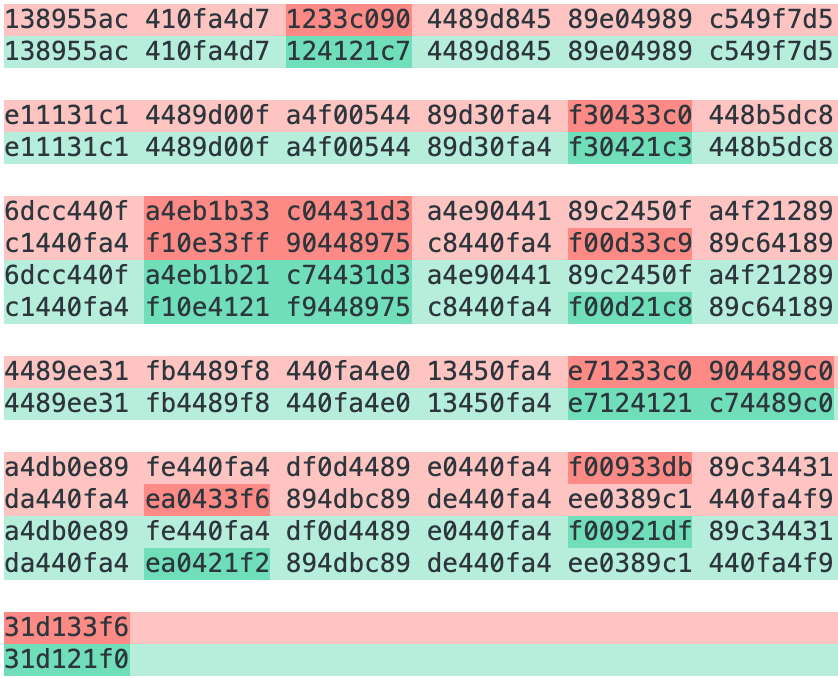
\includegraphics[width=0.45\textwidth]{report/figures/diff.png}}
\caption{Diff: original binary (green) and modified binary (red).}
\label{fig:diff}
\end{figure}

It turns out that the non-linearity of the feedback function can be removed by modifying as few as 15 bytes using the method described in Equation \ref{form:and}. The modification of the binary can be seen in Figure \ref{fig:mod-asm-imp}. The authors note that the cryptanalysis as described in Section \ref{sec:cryptanalysis} follows in a similar fashion but requires a few extra terms in the equation.

\begin{figure}[H]
\begin{lstlisting}[style=asm, frame=tlrb]
<_ECRYPT_ivsetup>
and    %esi,%esi    21 f6
and    %esi,%esi    21 f6
and    %eax,%eax    21 c0

<_ECRYPT_process_bytes>
and    %eax,%eax    21 c0
and    %ebx,%ebx    21 db 
and    %eax,%eax    21 c0
nop                 90

and    %edi,%edi    21 ff
nop                 90
and    %ecx,%ecx    21 c9
and    %eax,%eax    21 c0
nop                 90
\end{lstlisting}
\caption{Modified Assembly Code (improved)}\label{fig:mod-asm-imp}
\end{figure}

After injecting the faults as described above, both the keystream generation algorithm as well as the key and IV setup are no longer non-linear [See Figure \ref{fig:modified}]. 

\subsection{Keystream Generation}

After the injecting the faults the keystream remains a linear combination of the three registers, $t_1 \oplus t_2 \oplus t_3 = z_i$. However, at each clock cycle, three bits are updated using a, now, linear feedback function, whist one output bit $z_i$ is obtained [See Algorithm \ref{alg:mod-key} and Figure \ref{fig:modified}].

\begin{algorithm}[H]
\begin{algorithmic}[1]
\For{$i=1$ to $N$} \Comment{$N\leq 2^{64}$}
\State $t_1 \gets s_{66} + s_{93}$
\State $t_2 \gets s_{162} + s_{177}$
\State $t_3 \gets s_{243} + s_{288}$
\State
\State $z_i \gets t_1 + t_2 + t_3$
\State
\State $t_1 \gets t_1 + s_{171}$
\State $t_2 \gets t_2 + s_{264}$
\State $t_3 \gets t_3 + s_{69}$
\State
\State $(s_1,s_2,\dots,s_{93}) \gets (t_3,s_1,\dots,s_{92})$
\State $(s_{94},s_{95},\dots,s_{177}) \gets (t_1,s_{94},\dots,s_{176})$
\State $(s_{178},s_{179},\dots,s_{288}) \gets (t_2,s_{178},\dots,s_{287})$
\EndFor
\end{algorithmic}
\caption{Modified Keystream Generation} \label{alg:mod-key}
\end{algorithm}

\subsection{Key and IV Setup}

The key and IV setup proceeds as before, requiring $4*288=1152$ steps and giving no output bits [See Algorithm \ref{alg:mod-iv}].

\begin{algorithm}[H]
\begin{algorithmic}[1]
\State $(s_1,s_2,\dots,s_{93}) \gets (K_1,\dots,K_{80},0,\dots,0)$
\State $(s_{94},s_{95},\dots,s_{177}) \gets (IV_1,\dots,IV_{80},0,\dots,0)$
\State $(s_{178},s_{179},\dots,s_{288}) \gets (0,\dots,0,1,1,1)$
\State
\For{$i=1$ to $4\cdot288$}
\State $t_1 \gets s_{66} + s_{93} + s_{171}$
\State $t_2 \gets s_{162} + s_{177} + s_{264}$
\State $t_3 \gets s_{243} + s_{288}+ s_{69}$
\State
\State $(s_1,s_2,\dots,s_{93}) \gets (t_3,s_1,\dots,s_{92})$
\State $(s_{94},s_{95},\dots,s_{177}) \gets (t_1,s_{94},\dots,s_{176})$
\State $(s_{178},s_{179},\dots,s_{288}) \gets (t_2,s_{178},\dots,s_{287})$
\EndFor
\end{algorithmic}
\caption{Modified Key and IV Setup} \label{alg:mod-iv}
\end{algorithm}

\begin{figure}[H]
\centering
\includestandalone[width=0.45\textwidth]{figures/modified}
\caption{Modified Trivium}
\label{fig:modified}
\end{figure}

\section{Cryptanalysis}\label{sec:cryptanalysis}

In order to obtain the key from the ciphertext, the cryptanalysis is done as follows. If the keystream $ks$ was not directly observed, it can be obtained from the ciphertext $ct$ of a known plain text $pt$. 
$$ct_i = ks_i \oplus pt_i$$
$$ks_i = ct_i \oplus pt_i = ks_i \oplus pt_i \oplus pt_i$$
Once the keystream has been obtained, the cryptanalysis proceeds in two stages; obtaining the keystream from the initial state and finally extracting the key from the initial state.

\subsection{Initial State from Keystream}

After recording $\alpha$ bits of the keystream we set up the following system of linear equations, where $a,b$ and $c$ each denote one of the three LFSRs, $s_1,\dots,s_{288}$ are the state variables, and $z_1,\dots,z_{\alpha}$ are the keystream bits. 
\resizebox{.45\textwidth}{!}{ 
${\displaystyle {\overset {\alpha\times 288{\text{ matrix}}}
{\begin{bmatrix}
a_{1,1}& \dots & a_{1,93} & b_{1,1} & \dots & b_{1,84} & c_{1,1} & \dots & c_{1,111}\\
\vdots &  & \vdots & \vdots &  & \vdots & \vdots &  & \vdots\\
a_{i,1}& \dots & a_{i,93} & b_{i,1} & \dots & b_{i,84} & c_{i,1} & \dots & c_{i,111}\\
\vdots &  & \vdots & \vdots &  & \vdots & \vdots &  & \vdots\\
a_{\alpha,1}& \dots & a_{\alpha,93} & b_{\alpha,1} & \dots & b_{\alpha,84} & c_{\alpha,1} & \dots & c_{\alpha,111}\\
\end{bmatrix}}}
{\overset {288\times 1{\text{ matrix}}}
{\begin{bmatrix}
s_{1} \\
\vdots \\
s_{288} \\
\end{bmatrix}}}
=
{\overset {\alpha\times 1{\text{ matrix}}}
{\begin{bmatrix}
z_{1} \\
\vdots \\
z_{i} \\
\vdots \\
z_{\alpha} \\
\end{bmatrix}}}}
$}

\subsection{Key from Initial State}

The initial state is then expressed as a system of 288 linear equations, made up from 80 unknown bits from the key, 80 known bits from the IV, 125 bits set to 0, and three bits set to 1. A linear system with $k$ unknown variables can be solved using Gaussian elimination in time $\mathcal{O}(k^3)$. Thus, finding the solution takes at most $80^{3}$ operations. We note that there is no need to use asymptotically faster algorithms such as those described in \cite{gauss}, since we are only dealing with 80 variables and such methods would in fact be slower for systems of this size.
 
\section{Summary and Future Work}

In this paper we presented a non-invasive attack on the Trivium stream cipher. The attack introduces stuck-at-0 faults at the outputs of AND gates by modifying only 21 bytes in the binary code. We note that it is also possible to introduce a stuck-at-1 fault modifying as few as 15 bytes.Our attack reduces the non-linear feedback function to a linear one, making retrieval of the internal state and key tractable.

A way to further develop the attack would be to use a combination of our proposed stuck-at-0 fault injection along with another previously studied attack. One such possibility would be to mount the GD attack by \cite{Rohani2010} as discussed in Section \ref{sec:previous-work} on top of our fault injection. This could potentially further improve the attack, although this remains to be investigated. In this paper, we have focused solely on the software implementation of Trivium. Since Trivium was selected as part of the hardware portfolio of the eSTREAM project, it would make sense to test the attack on a hardware implementation of the cipher. Such an attack would similarly aim to modify the VHDL code in targeted positions, and then load the faulty design onto the FPGA. It is likely that a hardware based attack would have the same outcome as in software.

\section*{Acknowledgement}

I would like to thank Elena Dubrova for the idea and her support throughout this project. I'd also like to extend my gratitude towards Per Austrin for making this project possible as well as Daniel Skantz for the invaluable conversations.

\bibliographystyle{IEEEtran}
\bibliography{IEEEabrv,bibl-rep}
\nocite{*}

\end{document}
